%# -*- coding: utf-8-unix -*-

\raggedbottom
\chapter{基础算法与优化思路}
\label{chap:algorithm}

\section{引言}
经典的非交互式差分隐私匿名算法DiffGen是本课题优化算法设计的基础。本章节有针对性地对DiffGen算法进行介绍分析,并揭示其缺陷的本质模型为频率矩阵加噪模型。接下来探讨针对一维直方图发布方式的优化方案$BoostH$,总结其应用特性,并分析与DiffGen的联系和启发思路,为接下来的优化算法做铺垫。
%这也给频率矩阵模型问题提供了解决方案,并结合DiffGen算法,为接下来的优化算法做铺垫。

\section{基础算法概览}

DiffGen算法是由Mohammed等人于2011年提出的一个非交互式差分隐私匿名算法\supercite{DiffGen},基于分类树结构和指数机制构建重匿名数据集,其性能优于SuLQ-basedID3和DiffP-C4.5。
%本节的示例均基于例\ref{chap3_exmp}的背景,表述如下:
\begin{exmp}
	\label{chap3_exmp}
	某公司有8位应聘者,对“国籍”、“年龄”以及是否被录用统计如表\ref{chap3_table}(a),类属性为“是否被录用”。
\end{exmp}

\begin{table}[!hpb]
	\label{chap3_table}
	\centering
		\bicaption[tab:firstone]{表}{应聘者统计表}{Table}{The statistical table for candidates}
	\subtable[统计表]{
		\begin{tabular}{|c|c|c|}
			\hline
			$\textbf{国籍}$ & $\textbf{年龄}$ & $\textbf{是否被录用}$ \\
			\hline
			中国 & 18 & 否 \\
			\hline
			蒙古 & 21 & 是 \\
			\hline
			伊朗 & 27 & 否 \\
			\hline
			以色列 & 35 & 否 \\
			\hline
			以色列 & 29 & 是 \\
			\hline
			中国 & 39 & 是 \\
			\hline
			蒙古 & 22 & 否 \\
			\hline
			中国 & 28 & 否 \\
			\hline
		\end{tabular}}
		\qquad
		\subtable[泛化处理后的统计表]{%
			\begin{tabular}{|c|c|c|}
				\hline
				$\textbf{国籍}$ & $\textbf{年龄}$ & $\textbf{类属性计数(录用分布)}$ \\
				\hline
				东亚 & [15-25) & 3 (1是2否) \\
				\hline
				东亚 & [25-40) & 2 (1是1否) \\
				\hline
				西亚 & [15-25) & 0 (0是0否) \\
				\hline
				西亚 & [25-40) & 3 (1是2否) \\
				\hline
			\end{tabular}}
		\end{table}

\subsection{泛化技术与匿名树}

泛化技术是匿名算法实现的关键技术,在DiffGen中通过匿名树(Taxonomy tree)来组织每个属性下属性值的匿名层级关系,如图\ref{fig3:taxonomy}所示。原属性作为叶节点,通过指定更一般的泛化域(Dom),自底向上地构建匿名树,如中国与蒙古的泛化域为东亚。
对于离散属性(Categorical attribute)如“国籍”,采用抽取共性的方式进行逐层泛化;对于连续属性(Numerical attribute)如“年龄”,通过更大的连续区间进行泛化。表\ref{chap3_table}(b)是泛化处理后的统计结果。
从根节点自顶向下来看,匿名树定义了一套划分规则,指导每个泛化属性如何分裂;从叶节点自底向上来看,匿名树定义了一套抽象规则,显示了父子节点间的泛化包含关系。
%显然匿名树中的属性值是不重复。

匿名规则需要数据发布者自己定义,算法读取语义文件并构建匿名树作为属性分裂时的划分依据。匿名树最底层的非叶子节点用气泡框标识,表示最“细”的发布属性值,最多发布到此为止。

\begin{figure}[!htp]
	\centering
	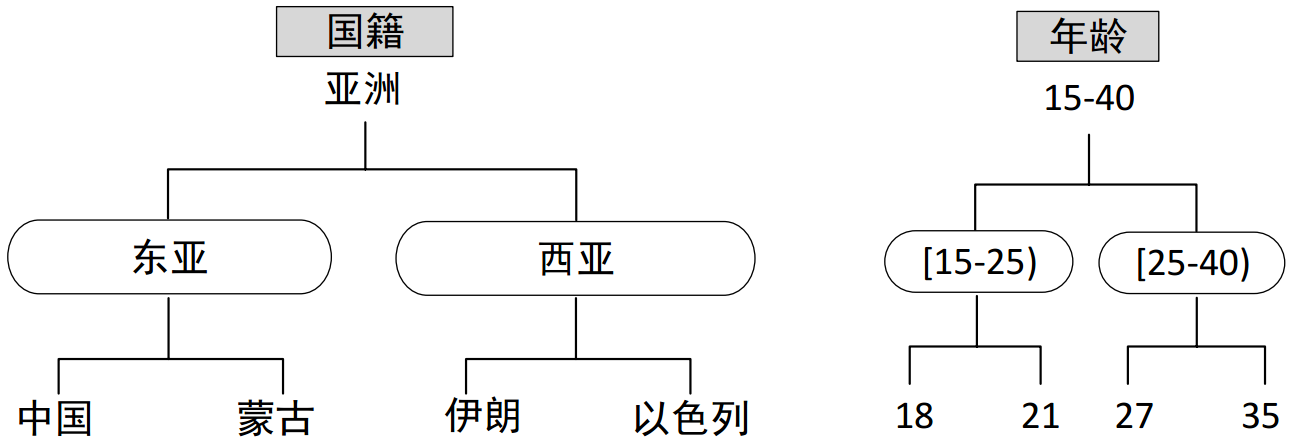
\includegraphics[width=5in]{chap3/taxonomy}
	\bicaption[fig3:taxonomy]{图}{属性“国籍”和“年龄”的匿名树}{Fig.}{The taxonomy tree for 'Country' and 'Age'}
\end{figure}


\subsection{算法概述}

面向分类应用的非交互式差分隐私匿名算法DiffGen主要的流程为:(1)为每个属性定义匿名树语义文件,并定义树高。(2)基于决策树算法构建“DiffGen分类树”并逐层划分数据集。(3)由叶节点的类属性计数生成发布数据集。
整个流程伪代码\ref{total_diffgen}概括如下,其中,“DiffGen分类树”是数据集划分、属性选择的基础结构。

\begin{algorithm}[H]
	\caption{DiffGen算法流程} 
	\label{total_diffgen}
	\begin{algorithmic}[1]
		\REQUIRE 隐私代价$\varepsilon$,树高$Hight$,数据集,匿名树集合。
		\ENSURE 发布数据集。
		\STATE 定义合理数据结构处理数据集和匿名树森林,并建立相应联系
		\STATE 初始化分类树根节点,记当前树高为$h$
		\WHILE{$h++$ < $Hight$} 
		\STATE 基于决策树算法,逐层选择属性、分裂当前节点并划分父节点数据集,构建分类树。
		\ENDWHILE
		\STATE 在分类树叶子节点的类属性计数上添加拉普拉斯噪音,全局敏感性为1。
		\STATE 遍历叶节点,根据类属性计数值生成匿名化数据集
		\RETURN 发布数据集
	\end{algorithmic}
\end{algorithm}


\subsection{算法框架}

DiffGen算法依据匿名树的分裂规则,采用决策树算法通过指数机制逐层选择分裂属性,并作数据集划分,构建完整的分类树,最后在叶节点加噪并发布数据集。为了更清楚地展示这个过程以及理解DiffGen算法伪代码,继续使用前文公司应聘的例子做说明。

DiffGen算法以匿名树作为属性划分规则,采用决策树算法通过指数机制逐层选择分裂属性,并作数据集划分,构建完整的DiffGen分类树,最后在叶节点加噪并发布数据集。图\ref{fig3:diffgen}展示了例\ref{chap3_exmp}背景下的算法工作过程。算法\ref{diffgen}对DiffGen算法进行了完整描述,其中$Cut_{i}$表示在当分类树树高为i时,所有匿名树中可分裂的属性集合。如仅有根节点时,$Cut_{1}$=\{亚洲,[15-40)\};而选取分裂属性亚洲后,$Cut_{2}$=\{东亚,西亚,[15-40)\}。$u(D,\cdotp)$表示打分函数,$S(u)$为其全局敏感性。

\begin{algorithm}
	\caption{DiffGen算法} 
	\label{diffgen}
	\begin{algorithmic}[1]
		\REQUIRE 隐私代价$\varepsilon$,树高$Height$,数据集$D$。
		\ENSURE 新的匿名数据集$\hat{D}$。
		\STATE 初始化分类树根节点和$Cut_{i}$集合,此时i=1
		\STATE 按树高切割$\varepsilon$,统计连续属性个数为$A_{Pr}^{n}$,$\varepsilon$' $\leftarrow$ $\frac{\varepsilon}{2(|A_{Pr}^{n}|+2Hight)}$
		\STATE 对$Cut_{i}$里的每个连续属性$v_{n}$,计算其分裂点$p$,分裂点$p$的选中概率 $\wasypropto$ exp($\frac{\varepsilon\textasciiacute}{2S(u)}$$u(D,v_{n})$)
		\STATE 对所有的属性$v$, $\forall$$v$ $\in$ $Cut_{i}$,计算分值
		\FOR{i = 1 to $Hight$}
		\STATE 按分值选择属性$v$,$v$$\in$ $Cut_{i}$,且$v$的选中概率$\wasypropto$ exp($\frac{\varepsilon\textasciiacute}{2S(u)}$$u(D,v)$)
		\STATE 根据$v$的匿名树分裂节点$v$,$v$$\rightarrow$$child(v)$
		\STATE $Cut_{i}$ $\leftarrow$ $Cut_{i}$$ - $$v$,$Cut_{i}$ $\leftarrow$ $Cut_{i}$ $\cup$ $child(v)$
		\STATE 对$Cut_{i}$里的新出现的连续属性$v_{n}$,计算其分裂点$p$,分裂点$p$的选中概率 $\wasypropto$ exp($\frac{\varepsilon\textasciiacute}{2S(u)}$$u(D,v_{n})$)
		\STATE 对所有的属性$v$, $\forall$$v$ $\in$ $Cut_{i}$,更新分值
		\ENDFOR
		\RETURN 在叶子节点的数据项上,每个类属性计数为$C$,返回($C$+$\textit{Laplace}$(1/$\varepsilon$))
	\end{algorithmic}
\end{algorithm}


\begin{figure}[!htp]
	\centering
	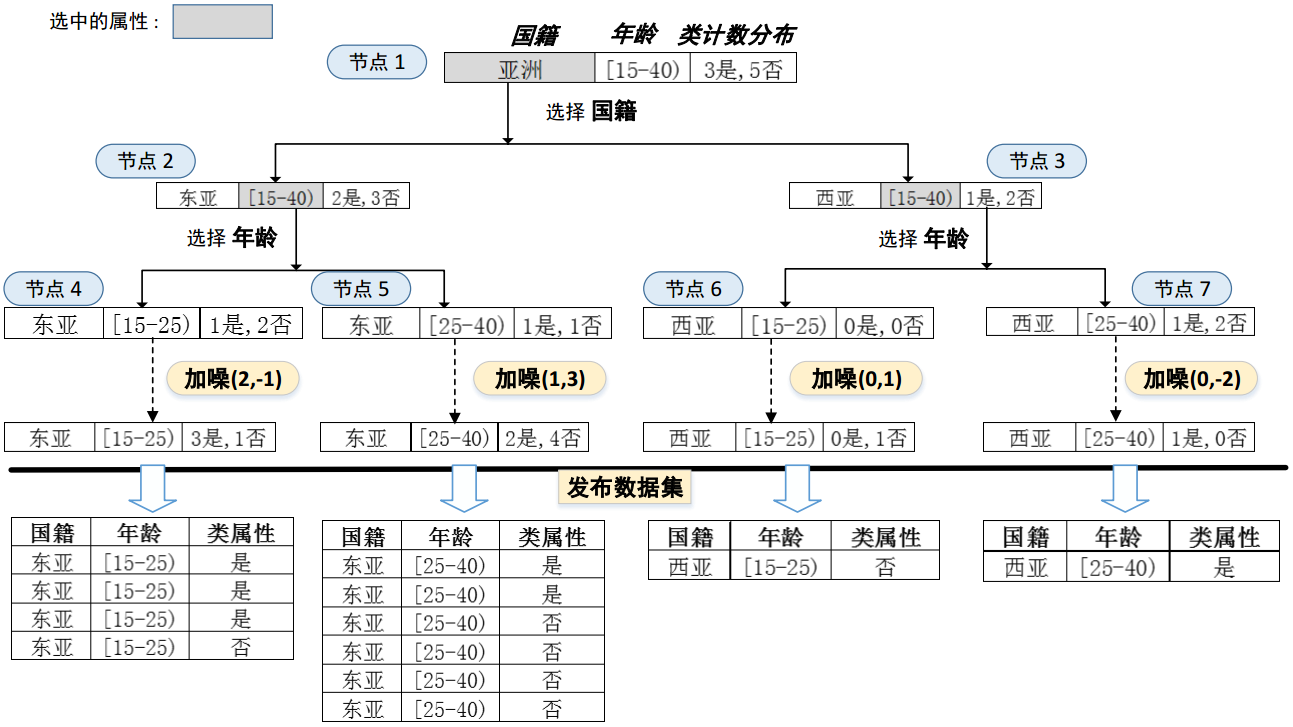
\includegraphics[width=6.2in]{chap3/diffgen}
	\bicaption[fig3:diffgen]{图}{基于DiffGen算法的数据集发布流程概述}{Fig.}{The release process for dataset based DiffGen}
\end{figure}

结合算法\ref{diffgen}与图\ref{fig3:diffgen},DiffGen的运行过程概括如下:

\begin{enumerate}
	\label{process}
	\item 事先定义DiffGen分类树的树高$Height$。在第1行做初始化,组合所有匿名树的根节点属性值作为分类树的根节点与$Cut_{i}$的初始值。在第2行对隐私预算按层切分,在每层选取分裂属性和处理连续属性分裂点时提供隐私保障。
	\item 在5-10行的每次迭代中,需要先对待选择属性集$Cut_{i}$的每个属性计算打分值并对连续属性进行处理,然后通过指数机制按概率挑选属性;在第8,9,10行为更新操作。
	\item 分裂节点的同时伴随着数据集的划分,节点上的数据项根据属性值包含关系,归入下层的相应节点。例如,节点1选出属性“国籍”,根据匿名树划分为“东亚”和“西亚”,生成节点2和节点3,同时节点1上的数据集也根据属性泛化关系并入相应的节点。
	\item 对节点来说,有两种情况不发生节点分裂:(a)到迭代上限,即树高$Height$。(b)选中属性在此节点的属性值是匿名树的最“细”划分限度——“气泡框”。
	\item 以图\ref{fig3:diffgen}以中间的粗直线为界,上半部分为完整的DiffGen分类树,下半部分为数据发布过程。算法的第12行在每个叶节点类属性计数上添加独立的拉普拉斯噪音,并返回。最后发布统计情况,发布的新数据集如表\ref{chap3_table2}的(a)(b)(c)(d)所示。
\end{enumerate}

\begin{table}[!hpb]
	\label{chap3_table2}
	\centering
	\bicaption[tab:firstone]{表}{DiffGen算法处理后的发布数据集}{Table}{The realesed dataset after DiffGen}
	\subtable[数据项1]{
		\begin{tabular}{|c|c|c|}
			\hline
			$\textbf{国籍}$ & $\textbf{年龄}$ & $\textbf{是否被录用}$ \\
			\hline
			东亚 & [15-25) & 是 \\
			\hline
			东亚 & [15-25) & 是 \\
			\hline
			东亚 & [15-25) & 是 \\
			\hline
			东亚 & [15-25) & 否 \\
			\hline
		\end{tabular}}
		\qquad
		\subtable[数据项2]{%
		\begin{tabular}{|c|c|c|}
			\hline
			$\textbf{国籍}$ & $\textbf{年龄}$ & $\textbf{是否被录用}$ \\
			\hline
			东亚 & [25-40) & 是 \\
			\hline
			东亚 & [25-40) & 是 \\
			\hline
			东亚 & [25-40) & 否 \\
			\hline
			东亚 & [25-40) & 否 \\
			\hline
			东亚 & [25-40) & 否 \\
			\hline
			东亚 & [25-40) & 否 \\
			\hline
		\end{tabular}}
		\qquad
		\subtable[数据项3]{%
		\begin{tabular}{|c|c|c|}
			\hline
			$\textbf{国籍}$ & $\textbf{年龄}$ & $\textbf{是否被录用}$ \\
			\hline
			西亚 & [15-25) & 否 \\
			\hline
		\end{tabular}}
		\qquad
		\subtable[数据项4]{%
		\begin{tabular}{|c|c|c|}
			\hline
			$\textbf{国籍}$ & $\textbf{年龄}$ & $\textbf{是否被录用}$ \\
			\hline
			西亚 & [25-40) & 是 \\
			\hline
		\end{tabular}}
\end{table}


\subsection{算法缺陷}

根据DiffGen分类树的构建方法,落在每个叶节点中的数据集拥有相同的属性值分布,最终发布的数据集就是每个叶节点上的数据分布情况。如图\ref{fig3:diffgen}的下半部分所示,这就是一个二维类属性分布的频率矩阵。显然,DiffGen往叶节点的每个类分布加噪的方式其实就等同于频率矩阵加噪模型中往每个行项加噪的做法。

在查询应答模式上,DiffGen采用的是线性累加的应答查询模式$LinearR$。首先DiffGen的叶节点集满足差分隐私的水平组合性质(见\ref{parallel}节,论文\parencite{DiffGen}已证明),叶节点间均两两不相交(证明在下个章节),因此叶节点上的加噪和应答是相互独立的,其拉普拉斯噪音的敏感性为一常量。其次,发布数据集的结构决定了基于行项的应答处理模式---直接发布含噪的N维类属性分布频率矩阵。
例如,在发布数据集上运行决策树分类算法产生范围计数查询需求,计算总熵值时需要对全属性分布的计数情况进行累加计算,此时[数据项\{1,2,3,4\}]需线性叠加运算;当计算“东亚”的熵值时,需要[数据项\{1,2\}]的线性叠加运算。

可见,在范围查询需求的应用中,DiffGen模型的缺陷本质和前文所讨论的频率矩阵加噪模型是一致的,以行项级别粒度的加噪方式与线性累加的应答查询模式会严重制约发布数据的可用性。


\section{一致性特性}

Michael Hay等人提出了利用一致性约束提升直方图方式(universal histogram)发布数据可用性的方法\supercite{boosting},为了书写方便本文称此优化方法为$BoostH$(boost histograms)。$BoostH$并未减少噪音量,而是通过对噪音分布的后置求精处理,使得对于任意范围的查询请求,应答结果均具有较高的准确度及可用性。其优化方案的一致性约束思路是本课题算法设计的基础。针对面向分类应用的范围计数查询需求,本节分析它与DiffGen算法的联系并总结启发思路。

\subsection{直方图发布方式}  %要说一下 DiffGen的频率矩阵加噪模型具有一维直方图特性!!!

以经典的LP\supercite{Dwork Calibrating}方法为例。直方图发布方式使用“分箱(Bin)”思想:先将属性值范围切割成若干个箱子,然后将数据集根据属性值放入不同的箱子构成一直方图,最后在每个柱状条(箱子)的计数上添加满足差分隐私的噪音,并发布数据。

在数据集$D$的直方图中,有$n$个柱状条,每个柱状条的属性值范围为$Bin_{i}$,其计数为$C(Bin_{i})$,加噪后计数为$\tilde{C}(Bin_{i})$,则一维直方图的数据发布格式$L_{unit}$与$\tilde{L}_{unit}$为
\[
\begin{split}
	L_{unit} = \{C(Bin_{1}),C(Bin_{2}),...,C(Bin_{n})\}\\
	\tilde{L}_{unit} = \{\tilde{C}(Bin_{1}),\tilde{C}(Bin_{2}),...,\tilde{C}(Bin_{n})\}	
\end{split}
\]
根据表\ref{chap3_table}(a)的“年龄”属性统计情况构建直方图\ref{fig3:histogram},“人数”表示该年龄段参加应聘的总人数。将年龄值范围[15-40]以5为间距切割成5个“箱子”,每条数据根据年龄值归入相应的柱状条中。最后,在每个柱状条上添加拉普拉斯噪音并发布数据,其中$L_{unit} = \{C(Bin_{15-19}),C(Bin_{20-24}),C(Bin_{25-29}),C(Bin_{30-34}),C(Bin_{35-40})\}$ = $\{1,2,3,0,2\}$%由于柱状条的计数分布是相互独立的,因此噪音的全局敏感性为1。

\begin{figure}[!htp]
	\centering
	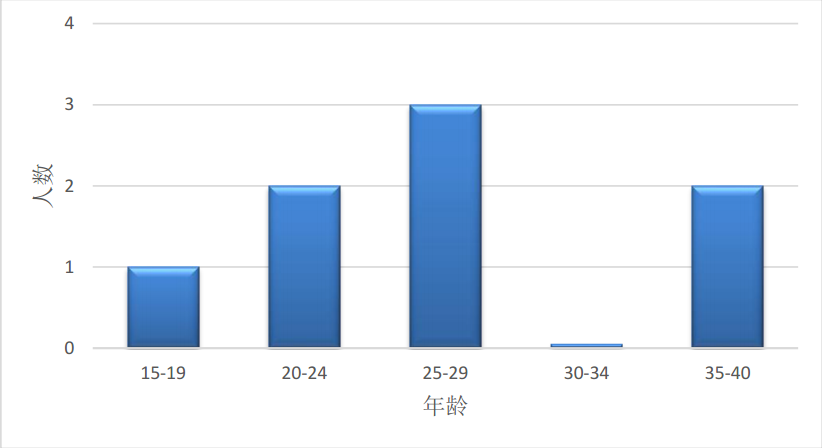
\includegraphics[width=5in]{chap3/histogram}
	\bicaption[fig3:histogram]{图}{属性“年龄”的直方图显示}{Fig.}{The Histogram of attribute 'Age'}
\end{figure}

差分隐私中的直方图发布方式对于单位长度(Unit length)的查询能提供较好的支持,每个柱状条代表单位长度的计数情况,直接返回即可。但是对于范围查询请求来说,只能采用线性叠加的查询应答模式$LinearR$。由于每个柱状条的属性值区间是相互独立的,并且全局敏感性为一常量,因此直方图模型也遇到了频率矩阵加噪模型一样的问题。

\subsection{一致性特性}
\label{LP_publish}

就差分隐私直方图发布方式在范围查询中的噪音线性叠加问题,$BoostH$通过树状的辅助结构$BoostTree$,改变线性叠加的查询应答模式为树结构相关的搜索应答模式,并通过利用一致性约束对噪音分布进行优化。

图\ref{fig3:histogram}的“年龄”直方图发布格式虽然是基于单位长度柱状条分布的$\tilde{L}_{unit}$,但是不同的年龄属性之间存在着一致性关系。图\ref{fig3:consistency}呈现了这种关系,归纳了“年龄”的树状辅助结构$BoostTree$。利用了泛化技术处理属性值区间,把单位长度柱状条作为叶节点,自底向上构建树结构,完成对直方图的转换。图中的标号A,B,C,D,E对应原先直方图中的单位柱状条。由于属性值区间的包含关系,此时可从树结构中的父子节点对得到以下的一致性关系等式,${\it{C}}_{a-b}$表示属性值区间[$a-b$]的计数值:
\begin{equation}
\label{consistent_equal}
\begin{split}
&{\it{C}}_{15-24} = {\it{C}}_{15-19}+{\it{C}}_{20-24}\\
&{\it{C}}_{25-34} = {\it{C}}_{25-29}+{\it{C}}_{30-34}\\
&{\it{C}}_{15-34} = {\it{C}}_{15-24}+{\it{C}}_{25-34}\\
&{\it{C}}_{15-40} = {\it{C}}_{15-34}+{\it{C}}_{35-40}
\end{split}
\end{equation}

\begin{figure}[!htp]
	\centering
	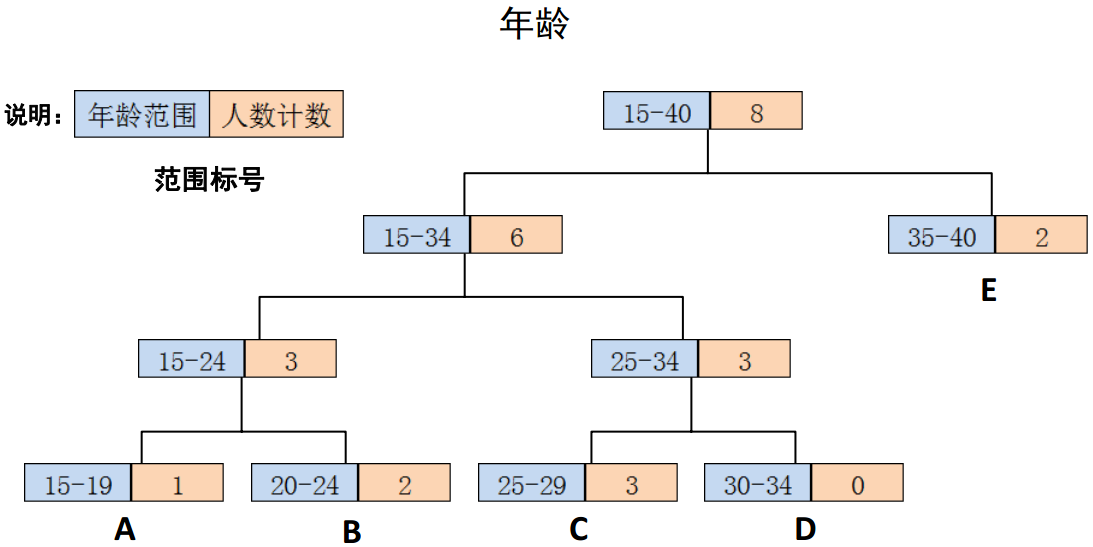
\includegraphics[width=5in]{chap3/consistency}
	\bicaption[fig3:consistency]{图}{属性“年龄”的树状组织结构"BoostTree"}{Fig.}{The tree-organization structure 'BoostTree' for attribute 'Age'}
\end{figure}

%在直方图方式中,通过{$\widetilde{C}$} = {\it{C}} + Laplace(1/$\varepsilon$)给每个单位柱状条加噪音,并以累加操作响应非单位长度的范围查询。如查询年龄为[15-34],则返回结果({$\widetilde{C}_{A}$}+{$\widetilde{C}_{B}$}+{$\widetilde{C}_{C}$}+{$\widetilde{C}_{D}$})。但是
此时,对于年龄区间[15-34]的查询,通过等式\ref{consistent_equal}可以看到,若能直接返回范围节点{$\widetilde{C}_{15-34}$},从噪音叠加次数上来看,显然优于原方案的单位长度节点累加$\{\tilde{C}(Bin_{15-19})+\tilde{C}(Bin_{20-24})+\tilde{C}(Bin_{25-29})+\tilde{C}(Bin_{30-34})\}$。由于噪音的随机性,虽然加噪后两种方案数值结果不一定能划等号,但至少可以提供选择min({$\tilde{C}_{15-34}$},{$\tilde{C}_{A}$}+{$\tilde{C}_{B}$}+{$\tilde{C}_{C}$}+{$\tilde{C}_{D}$})给用户。多种组合的选择无疑给发布数据带来了提升空间。

因此,初步想法是改变基于叶节点的加噪方式为遍布$BoostTree$上所有节点的加噪,即按某种节点遍历顺序发布树节点信息,然后对于范围查询偏向于返回范围节点的含噪计数值,或者直接发布整个节点集供用户挑选更优的组合。假设树上有$ntree$个节点,这种发布格式$\tilde{L}_{all}$为
\begin{equation}
\label{L_allnodes}
\tilde{L}_{all} = \{\tilde{C}_{1},\tilde{C}_{2},...,\tilde{C}_{ntree}\}
\end{equation}

此方案改变了原先$LinearR$的应答查询模式,除了单位长度节点外,通过提供范围节点的应答选择,达到优化噪音叠加问题的目的。
%因为一致性是属性值区间之间的内在属性,加噪操作改变的仅仅是数值。更具一般性,由于噪音数值的不确定性,我们可以选取min({$\widetilde{C}_{15-34}$},{$\widetilde{C}_{A}$}+{$\widetilde{C}_{B}$}+{$\widetilde{C}_{C}$}+{$\widetilde{C}_{D}$})作为应答返回,这无疑给发布数据提供了提升空间。

\subsection{BoostH的优化方案}
\label{BoostH}

但$\tilde{L}_{all}$的发布格式存在着两个弊端:
\begin{itemize}
	\item 给$BoostTree$的每个节点加噪之后,由于噪音的随机性使得节点间的一致性等式不再成立,例如绝大部分情况下{$\tilde{C}_{15-24}$}$ \neq ${$\tilde{C}_{15-19}$}+{$\tilde{C}_{20-24}$}。此时从数值上分辨不出节点间的一致性关系,因此无法挑选出多种应答方案,优化方案失效。
	\item 基于前一点的问题,只能通过其他的辅助方法告知树节点间的关系。这虽然能利用$BoostTree$的一致性特性,但泄露了树结构、内部节点等信息,发布数据集的安全性得不到保障。
\end{itemize}

因此$\tilde{L}_{all}$的发布方案不可行,但是其改变应答查询模式的思路是可取的。对于查询范围$Q_{query}$,新的应答查询模式为:寻找$BoostTree$中能够覆盖$Q_{query}$的最小节点集合作为应答结果。例如,在图\ref{fig3:consistency}中,当$Q_{query}$ = \{[15-29]\},则返回节点集\{$\tilde{C}_{15-24}$,$\tilde{C}_{25-29}$\}。此方法能够有效避免噪音的线性叠加现象,但需要重新设计节点的发布格式。

$BoostH$采用此应答查询模式,重定义了全局敏感性,然后基于$BoostTree$结构对噪音分布进行后置处理,使得$BoostTree$上的含噪叶节点间重新满足\ref{consistent_equal}的一致性等式关系。重获一致性意味着任何内部节点可通过叶节点的线性累加获得,因此采用仅发布单位长度数据项格式即可,也就是DiffGen和一维直方图的$\tilde{L_{unit}}$格式。

$BoostH$的这种方案解决了$\tilde{L}_{all}$的两大弊端。首先,重获一致性的$BoostTree$结构使得非叶结点的应答可通过叶节点数据项的叠加得到,这和直接返回范围节点的效果是一样的;并且,省去了寻找覆盖节点的过程,此时对叶节点的累加操作是与事先寻找覆盖集再累加的效果是一样的。其次,未暴露内部节点信息,不影响安全性。此外,$BoostH$给新的应答查询模式定义了全局敏感性,并且噪音的调整仅仅是数值处理,因此的调整算法及数据发布过程并不违背差分隐私定义。

这种基于一致性约束的噪音优化调整方案,能够用简单的直方图发布方式在范围查询需求中获得较准确的应答结果,有效地解决频率矩阵加噪模型中的噪音线性叠加问题,且不失安全保障力度。此方案在应用背景、问题模型等方面与DiffGen算法有着密切的联系,启发了课题算法的设计思路。

%通过基于一致性约束的噪音优化调整过程,$BoostH$采用简单的直方图发布方式在响应范围查询请求的同时,达到了减免噪音叠加与确保数据结构安全性的目的。
%同样对于频率矩阵加噪问题,$BoostH$通过先树状辅助结构改变加噪方式,然后利用一致性特性调整噪音分布达到优化发布数据准确度的效果,并且未改变数据发布格式。



\subsection{框架适用性探讨}

根据上一节的论述,本小节对$BoostH$的基于一致性约束的优化方案与基础算法DiffGen的联系和启发进行总结:
\begin{enumerate}
	\item 模型基础。$BoostH$的直方图发布模型和DiffGen模型具有相同的模型特征---一维直方图的计数统计特征。此模型的特点在于每个单位数据项仅代表一维属性范围,任意的范围查询能够通过若干个数据项的叠加覆盖到,区别于多维属性直方图由于数据项表示范围的局限而无法完全覆盖的问题。
	虽然DiffGen的每个数据项包含多个属性,但是分类树的父子节点间存在完整的泛化包含关系,对于所有属性区间的查询均可通过叶节点的组合给予应答,因此不存在无法覆盖查询范围的问题,具有一维直方图特征。
	%各属性的范围查询均可以通过节点叠加完成,因此从X轴上看是多个一维属性直方图的组合。
	对于多维类属性分布数据集,可拆分成多个一维类属性直方图。因此,在范围技术查询应用中,DiffGen应具有一维直方图特征。
	\item 问题背景。二者的性能瓶颈是相同的:均属于频率矩阵加噪模型问题。基于单位长度的加噪操作、采用$LinearR$的线性累加的应答查询模式,在面对范围计数查询需求时,存在着噪音等额叠加的本质问题。
	\item 优化思路。泛化技术和决策树分类方式决定了DiffGen分类树中存在一致性特性。匿名树的父子层级之间存在明确的泛化关系,使得一致性特性成了DiffGen分类树中父子节点间的固有属性。
	\item 差分隐私定义。应答查询模式的改变影响了全局敏感性,由于树状辅助结构的引入和一致性关系的存在,单位长度计数值之间再也不是相互独立的了——某一单位长度计数值的改变至少影响着它到根节点路径上的所有节点。因此,需要重定义全局敏感性。
	\item 数据发布格式。由于重获一致性与树结构信息保护的需要,用考虑采用原先的直方图数据发布格式,也就是DiffGen的叶节点发布格式。因为对DiffGen来说,分类树的非叶节点信息不仅揭露了分类树的属性选择和分类结构,更关键的是它揭示了算法中的匿名化技术细节。匿名化结构的暴露会从根本上破坏DiffGen算法的隐私保护意义。因此,原先的仅发布单位数据项的做法应予以推崇。
	
\end{enumerate}

基于以上总结,在下一章节将详细介绍DiffCon算法的设计及实现。